\documentclass[simplex.tex]{subfiles}
% NO NEED TO INPUT PREAMBLES HERE
% packages are inherited; you can compile this on its own
%\usepackage{caption}
%\usepackage{subcaption}
\usepackage{enumitem}  

\begin{document}
\subsection{Law of Large Graphs}
We note that low-rank methods can often be more easily interpreted. Moreover, eigenmode is observed among the embedded latent positions, with respect to different lobes in particular. This suggests to use low-rank methods from another perspective. 
For all the 70 different regions based on the Desikan atlas (35 for each hemisphere), each one is assigned to one of the 10 lobes (5 for each hemisphere), i.e. Frontal, Parietal, Occipital, Temporal, and other. And we do a permutation test as following.

70 vertices are connected spatially as in the Desikan atlas. Let the adjacency matrix of these 70 vertices to be $A$. $A_{ij} = 1$ means vertex $i$ and vertex $j$ are spatially connected. We say vertex $j$ is a neighbor of vertex $i$ if $A_{ij} = 1$. We define $l_i$ be the lobe i.d. for vertex $i$.

We define a uniform $1$-flip to be:
\begin{itemize}
\item Select a pair of adjacent vertices (vertex $i_1$ and vertex $j_1$) across the boundary of lobes uniformly, i.e. $A_{i_1 j_1} = 1$ and $l(i_1) \ne l(j_1)$;
\item Uniformly select another pair of adjacent vertices (vertex $i_2$ and vertex $j_2$ where $i_1 \ne i_2$ and $j_1 \ne j_2$) across the same boundary of lobes uniformly, i.e. $A_{i_2 j_2} = 1$ and $l(i_1) = l(i_2)$ and $l(j_1) = l(j_2)$;
\item Reassign vertex $j_1$ to lobe $l_{i_1}$ and reassign vertex $i_2$ to lobe $l_{j_2}$.
\end{itemize}

By the definition, after a uniform $1$-flip, the number of vertices in each lobe keeps the same, where only two vertices are changed to a different lobe.

We define a uniform $k$-flip to be:
\begin{itemize}
\item Sequentially run the uniform $1$-flip $k$ times.
\end{itemize}

Note that after a uniform $k$-flip, the number of vertices in each lobe still keeps the same.

Let $X = [X_1, \cdots, X_n]^{\top}$ be the latent positions, where $X_i$ is the latent position for vertex $i$ sampled from distribution $f$. Test statistic $T(X, l)$ is defined as:
\[
T(X, l) = \frac{\sum_{i \ne j, l(i) = l(j)} \|X_i - X_j \|_2}{\sum_{i \ne j, l(i) = l(j)} 1} -
\frac{\sum_{i \ne j, l(i) \ne l(j)} \|X_i - X_j \|_2}{\sum_{i \ne j, l(i) \ne l(j)} 1}
\]



$H_0$: Differences between latent positions within lobes are the same compared to across lobes, i.e. $E_f[T(X, l)] = 0$.

$H_A$: Differences between latent positions within lobes are smaller compared to across lobes, i.e. $E_f[T(X, l)] < 0$.

We ran 1000 simulations for each number of flips and plot the results for the permutation test as in Figure~\ref{fig:violin}. The x-axis represents the different number of flips, while the y-axis represents the measure according to the lobe assignment, i.e. within lobes distances minus the across lobe distances. The dashed line is the baseline for the measure based on the true lobe assignment without any flipping. As the number of flips increases, we can see a clear evidence that $H_0$ is rejected with respect to $H_A$. Thus the embedded latent positions based on the low-rank method reflect the eigenmode with respect to different lobes.

\begin{figure}	
\centering
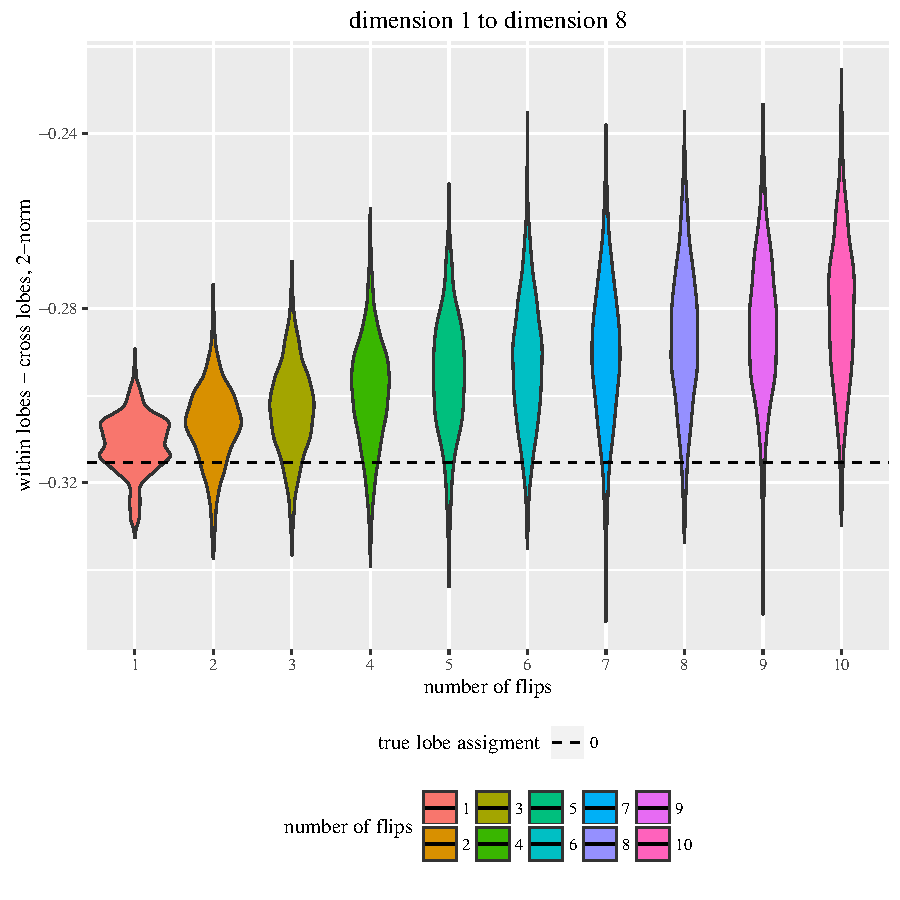
\includegraphics[height=.8\linewidth]{../../figs/violinplot_new_flip_2norm_1_8.pdf}
\caption{\textbf{Violin plot of the permutation test.} We ran 1000 simulations for each number of flips. The x-axis represents the different number of flips, while the y-axis represents the measure according to the lobe assignment, i.e. within lobes distances minus the across lobe distances. The dashed line is the baseline for the measure based on the true lobe assignment without any flipping. As the number of flips increases, we can see a clear evidence that $H_0$ is rejected with respect to $H_A$. Thus the embedded latent positions based on the low-rank method reflect the eigenmode with respect to different lobes.}
\label{fig:violin}
\end{figure}

%
\clearpage
\end{document}
